\documentclass[../INDE315.tex]{subfiles} 
\usepackage{fancyhdr}
\usepackage{graphicx}
\usepackage{amsmath}
\usepackage{mhchem}
\usepackage{amssymb}
\usepackage[margin=1in]{geometry}

\graphicspath{{./images/}}

\title{UW IND E 315 Notes}
\author{Anthony Le}

\begin{document}

\pagestyle{fancy}
\fancyhead{}
\fancyhead[R]{UW IND E 315}
\fancyhead[L]{Anthony Le}

\fancyhead[C]{Chapter 4 - Continuous Distribution}

\section*{Chapter 4 - Continuous Distribution}

\subsection*{Chapter 3 Recap}
Recall - Random Variable (rv) and Probability Distribution:
\begin{enumerate}
    \item \emph{Discrete} rv's have a \emph{countable} range
        \begin{enumerate}
            \item Ex - counts, integrers, natural numbers
        \end{enumerate}
    \item \emph{Continuous} rv's have an \emph{uncountable} range
        \begin{enumerate}
            \item Ex - length, weight, volume
        \end{enumerate}
    \item The probability distribution of a rv X is a description of the probabilities associated with the possible values of X.
        \begin{enumerate}
            \item Disrete probability distributions (Chapter 3)
            \item Continuous probability distributions (Chapter 4)
        \end{enumerate}
\end{enumerate}

\subsection*{Probability Distributions and Probability Density Functions (4.1)}
\subsubsection*{Probability Density Function (4.1)}

\begin{defn}
    \textbf{Probability Density Function (PDF)} \\
    \textbf{General} - Describes the probability distribution of a \textbf{continuous} rv $X$ \\
    ex: 
    \begin{center}
        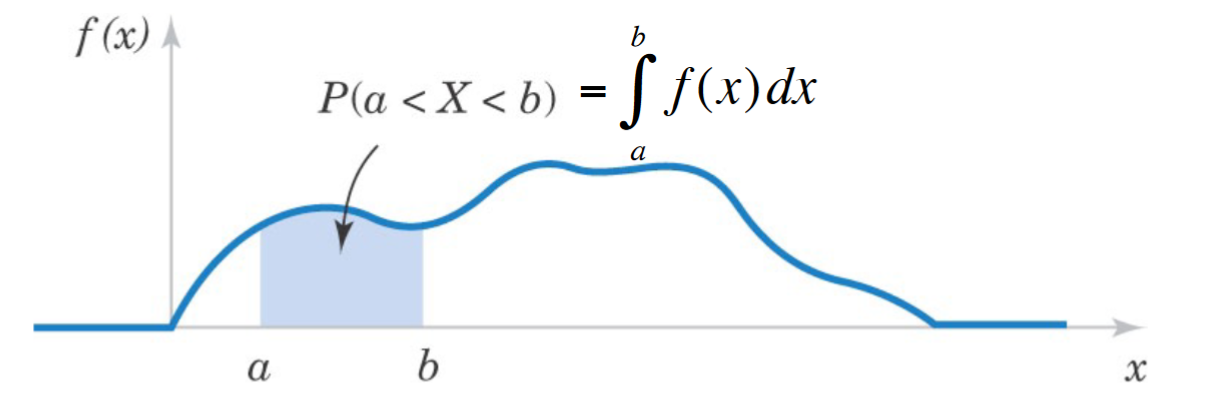
\includegraphics[width = 8cm]{Ch41_ProbabilityDensity}
    \end{center}
    ie in this case, the integral of $f(x)$ describes the area under the curve, or the probability occurring. \\
    \textbf{Formulaic} - For a \textbf{continuous} random variable $X$, a probability density function is a function such that:
    \begin{enumerate}
        \item $f(x) \geq 0$
        \item $\int_{- \infty}^{\infty}f(x) dx = 1$ 
        \item $P(a \leq X \leq b) = \int _a ^b f(x) dx$
    \end{enumerate}
\end{defn}

\subsubsection*{Example 4-1: Electric Current}
\begin{exmp} Example 4-1a: Electric Current \\
    Givens:
    \begin{enumerate}
        \item $X$ is a continuous random variable for the current in a thin copper wire in milliamperes (mA).
        \item Assume that the range for X is [4.9,5.1] mA and f(x)=5 for $4.9 \leq x \leq 5.1$
        \item What is the probability that a current is less than 5 mA?
    \end{enumerate}
    \begin{center}
        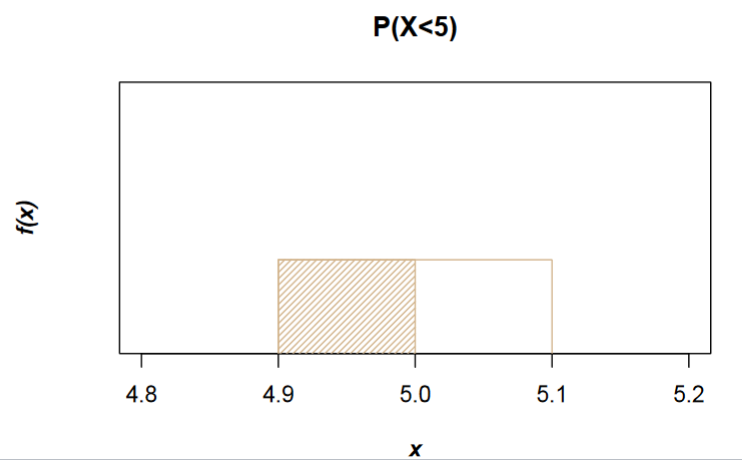
\includegraphics[width = 6cm]{Ch4Example1a}
    \end{center}
\end{exmp} 
Solve:
\begin{enumerate}
    \item Finding $P(X \leq 5)$
        \begin{equation*}
            \begin{aligned}
                P(a \leq X \leq b) &= \int _a ^b f(x) dx \\
                P(4.9 \leq X \leq 5) &= \int _{4.9} ^{5} 5 dx \\
                            &= \left. 5x \right|^{5}_{4.9} = 5(5) - 5(4.9) \\
                            &= 0.5
            \end{aligned}
        \end{equation*}
\end{enumerate}
\begin{exmp} Example 4-1b: Electric Current \\
    Givens:
    \begin{enumerate}
        \item What is the probability that a current will be between 4.95 and 5.1?
    \end{enumerate}
    \begin{center}
        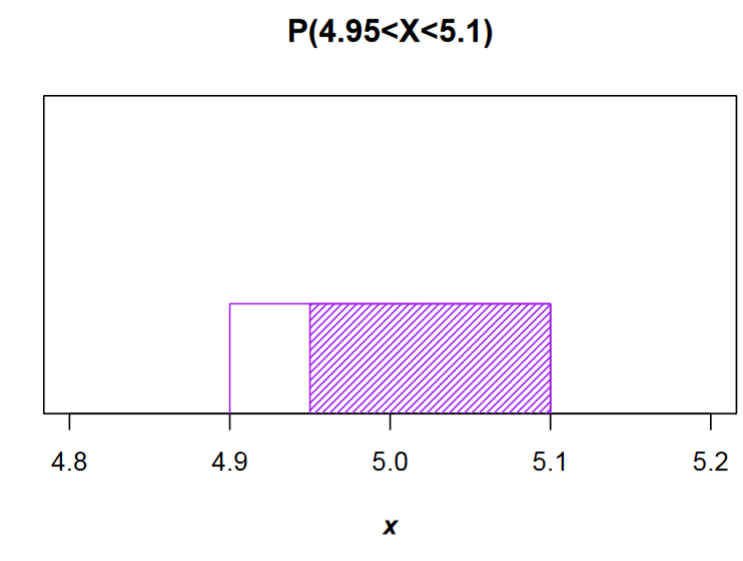
\includegraphics[width = 6cm]{Ch4Example1b}
    \end{center}
\end{exmp}
Solve: 
\begin{enumerate}
    \item Finding $P(4.95 \leq X \leq 5.1)$
        \begin{equation*}
            \begin{aligned}
                P(a \leq X \leq b) &= \int _a ^b f(x) dx \\
                P(4.95 \leq X \leq 5.1) &= \int _{4.95} ^{5.1} 5 dx \\
                            &= \left. 5x \right|^{5.1}_{4.95} = 5(5.1) - 5(4.95) \\
                            &= 0.75
            \end{aligned}
        \end{equation*}
\end{enumerate}

\subsubsection*{Example 4-2: Hole Diameter}
\begin{exmp} Example 4-2: Hole Diameter \\
    Givens:
    \begin{enumerate}
        \item $X$ is the diameter of a hole drilled in a sheet metal component.
        \item Target diameter = 12.5 mm.
        \item Distribution of X can be modeled by $f(X) = 20 e^{-20(x-12.5)}$.
        \item If a part with a diameter larger than 12.60 mm is scrapped, what proportion of parts is scrapped?
    \end{enumerate}
    \begin{center}
        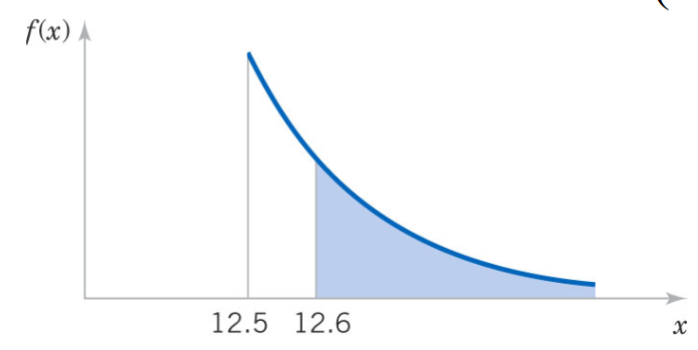
\includegraphics[width = 6 cm]{Ch4Example2}
    \end{center}
\end{exmp}
Solve:
\begin{enumerate}
    \item Finding $P(X > 12.60)$
        \begin{equation*}
            \begin{aligned}
                P(a \leq X \leq b) &= \int _a ^b f(x) dx \\
                P(\infty \geq X \geq 12.6) &= \int _{12.60} ^{\infty} 20 e^{-20(x-12.5)} dx \\
                            &= \left. -e^{-20(x-12.5)} \right|_{12.60} ^{\infty} \\
                            &= 0.135
            \end{aligned}
        \end{equation*}
\end{enumerate}

\subsection*{Cumulative Distribution Functions (4.2)}
\begin{defn}
    \textbf{Cumulative Distribution Function (CDF)} \\
    For a \textbf{continuous} random variable $X$, the CDF is,
    \begin{equation*}
        \begin{aligned}
            F(x) = P(X \leq x) = \int ^x _{-\infty} f(u) du \quad \text{for $-\infty < x < \infty$}
        \end{aligned}
    \end{equation*}
\end{defn}

\subsubsection*{Example 4-3: Electric Current (CDF)}
\begin{exmp} Example 4-3: Electric Current
    Based on Ex 4-1 (uniform distribution where $f(x) = 5$), the CDF consists of 3 expression to cover the entire real number line.
    \begin{center}
        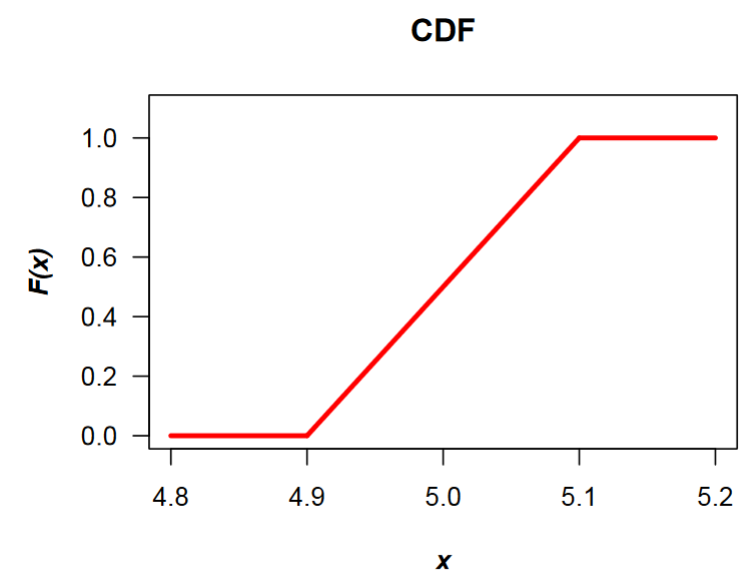
\includegraphics[width = 6 cm]{Ch4Example3}
    \end{center}
\end{exmp}
Solve:
\begin{equation*}
    \begin{aligned}
        F(x) = 
            \begin{cases}
                0 & x < 4.9 \\
                5x - 24.5 & 4.9 \leq x \leq 5.1 \\
                1 & 5.1 \leq x 
            \end{cases}
    \end{aligned}
\end{equation*}


\subsubsection*{Example 4-2: Hole Diameter (CDF)}
\begin{exmp} Example 4-2: Hole Diameter (CDF)
    Based on Ex 4-2, $F(x)$ consists of two expressions. Find them.
    \begin{center}
        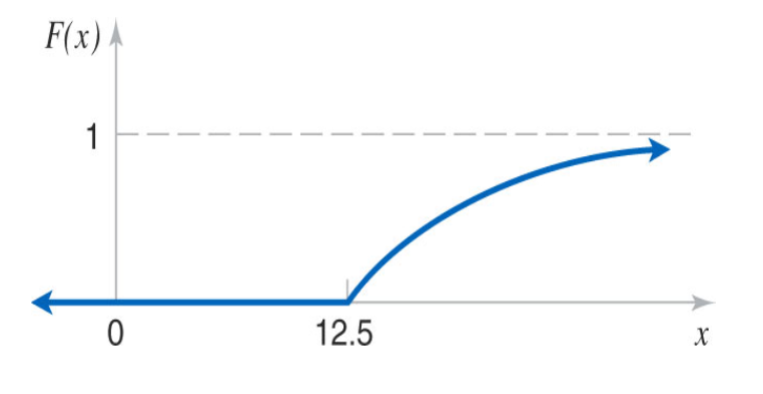
\includegraphics[width = 6cm]{Ch4Example2_CDF}
    \end{center}
\end{exmp}
\footnote{Thinking about this, im not really sure about how the CDFs and PDF/PMFs relate to each other. Like I think I get that CDFs should add up to 1, so you can just subtract the PDF/PMF's from 1 in order to get them to work - but im just not sure whether this is the right way to think about things.}
Solve:
\begin{enumerate}
    \item Finding F(x) for $x < 12.5$
        \begin{equation*}
            \begin{aligned}
                F(x) = 0 \quad \text{for $x < 12.5$}
            \end{aligned}
        \end{equation*}
    \item Finding F(x) for $x \geq 12.5$
        \begin{equation*}
            \begin{aligned}
                F(x) &= P(X \geq 12.5) = \int ^x _{12.5} 20 e^{-20(x-12.5)} dx \\
                    &= 1 - e^{-20(x-12.5)} \quad \text{for $x \geq 12.5$}
            \end{aligned}
        \end{equation*}
\end{enumerate}
\begin{equation*}
    \begin{aligned}
        F(x) = 
            \begin{cases}
                0 & \text{for $x < 12.5$} \\
                1 - e^{-20(x-12.5)} & \text{for $x \geq 12.5$}
            \end{cases}
    \end{aligned}
\end{equation*}

\subsubsection*{PDF vs. CDF}
\begin{enumerate}
    \item PDF ($f(X)$): the derivative of the cumulative distribution function (CDF) \\
        Given $F(x)$, $f(x) = \frac{dF(x)}{dx}$ as long as the derivative exists.
    \item CDF ($F(x)$): the definite integral of the probablity density function (PDF) from $-\infty$ to $x$. 
    \begin{equation*}
        \begin{aligned}
            F(x) = P(X \leq x) = \int ^{x}_{-\infty} f(u) du \quad \text{for $-\infty < x < \infty$}
        \end{aligned}
    \end{equation*}
\end{enumerate}

\subsection*{Mean and Variance of a Continuous Random Variable (4.3)}
\begin{defn}
    \textbf{Mean of a continuous random variable} \\
    Let $X$ be a continuous random variable with PDF, $f(x)$, then the mean is:
    \begin{equation*}
        \begin{aligned}
            \mu = E(X) = \int ^{\infty}_{-\infty} x f(x) dx
        \end{aligned}
    \end{equation*}  
\end{defn}

\begin{defn}
    \textbf{Variance of a continuous random variable} \\
    \begin{equation*}
        \begin{aligned}
            \sigma ^2 = V(X) &= \int ^{\infty}_{-\infty} (x - \mu)^2 f(x) dx  \\
                        &= \int ^{\infty}_{-\infty} x^2 f(x) dx - \mu ^2 
        \end{aligned}
    \end{equation*}
\end{defn}

\begin{defn}
    \textbf{Standard Deviation of a continuous random variable} \\ 
    \begin{equation*}
        \begin{aligned}
            \sigma = \sqrt{\sigma ^2 }
        \end{aligned}
    \end{equation*}    
\end{defn}
%//TODO - I like how every single formula is in the definitions here, so I think it might be worth going through and editing formula definitions to have them in a similar format to this

\begin{defn}
    \textbf{Expected value of a function ($h(X)$) of a continuous random variable X} \footnote{what is this h(x) we're working with? we haven't talked about this before}\\
    \begin{equation*}
        \begin{aligned}
            E(h(X)) = \int ^{\infty}_{-\infty} h(X) f(x) dx
        \end{aligned}
    \end{equation*}
    If $h(X) = aX + b$, then
    \begin{equation*}
        \begin{aligned}
             E(aX + b) = aE(X) + b
        \end{aligned}
    \end{equation*}
\end{defn}

\subsection*{Continuous Uniform Distribution (4.4)}
\begin{enumerate}
    \item Its PDF (probability density function) is defined as:
        \begin{defn}
            \textbf{PDF for a continuous uniform distribution} \\
            \begin{equation*}
                \begin{aligned}
                    f(x) = \frac{1}{b-a} \quad a \leq x \leq b
                \end{aligned}
            \end{equation*}
        \end{defn}
    \item Its mean is
        \begin{defn}
            \textbf{Mean for a continuous uniform distribution} \\
            \begin{equation*}
                \begin{aligned}
                    E(X) &= \int ^b _a \frac{x}{b-a} dx \\
                        &= \left. \frac{0.5x^2}{b-a} \right|^b _a \\
                    E(X) &= \frac{a + b}{2}
                \end{aligned}
            \end{equation*}
        \end{defn}
    \item Its variance is
        \begin{defn}
            \textbf{Variance for a continuous uniform distribution} \\
            \begin{equation*}
                \begin{aligned}
                    V(X) &= \int ^b _a \frac{(x - \frac{a+b}{2})^2}{b-a} dx \\
                        &= \left. \frac{(x - \frac{a+b}{2})^3}{3(b-a)} \right|^b _a \\
                    V(X) &= \frac{(b-a)^2}{12}
                \end{aligned}
            \end{equation*}
        \end{defn}
    \item Its CDF is
        \begin{defn}
            \textbf{CDF for a continuous uniform distribution} \\
            \begin{equation*}
                \begin{aligned}
                    F(x) &= \int ^x _a \frac{1}{b-a} \\
                        &= \left. \frac{u}{b-a} \right| ^x _a \\
                    F(x) &= \frac{x-a}{b-a} \\
                    F(x) &= 
                        \begin{cases}
                            0 & x < a \\
                            \frac{x-a}{b-a} & a \leq x < b \\
                            1 & b \leq x
                        \end{cases}
                \end{aligned}
            \end{equation*}
        \end{defn}
\end{enumerate}

\subsection*{Normal Distribution (4.5)}
Overview:
\begin{enumerate}
    \item Ubiquitous in nature due to the \emph{central limit theorem}
    \item Widely used for modeling by engineers
    \item The location and spread of the normal distribution are independently determined by mean ($\mu$) and standard deviation ($\sigma$)
\end{enumerate}

\subsubsection*{Normal Probability Density Function}
\begin{defn}
    \textbf{Probability Density Function (PDF) for normal distribution} \\
    A random variable X with a PDF\footnote{f(X) can't easily be integrated, so F(X) is available in Appendix A, Table III for \emph{standardized} normal}
    \begin{equation*}
        \begin{aligned}
            f(x) = \frac{1}{\sqrt{2 \pi} \sigma} e^{\frac{-(x-\mu)^2}{2\sigma ^2}}
        \end{aligned}
    \end{equation*}
    where:
    \begin{equation*}
        \begin{aligned}
            -\infty < x < \infty \\
            -\infty < \mu < \infty \\ 
            \sigma > 0
        \end{aligned}
    \end{equation*}
    is normal with parameters:
    \begin{equation*}
        \begin{aligned}
            E(X) = \mu \quad \text{and} \quad V(X) = \sigma ^2 
        \end{aligned}
    \end{equation*}
\end{defn}

\subsection*{Empirical Rule (describing standard deviations and probability)}
\begin{center}
    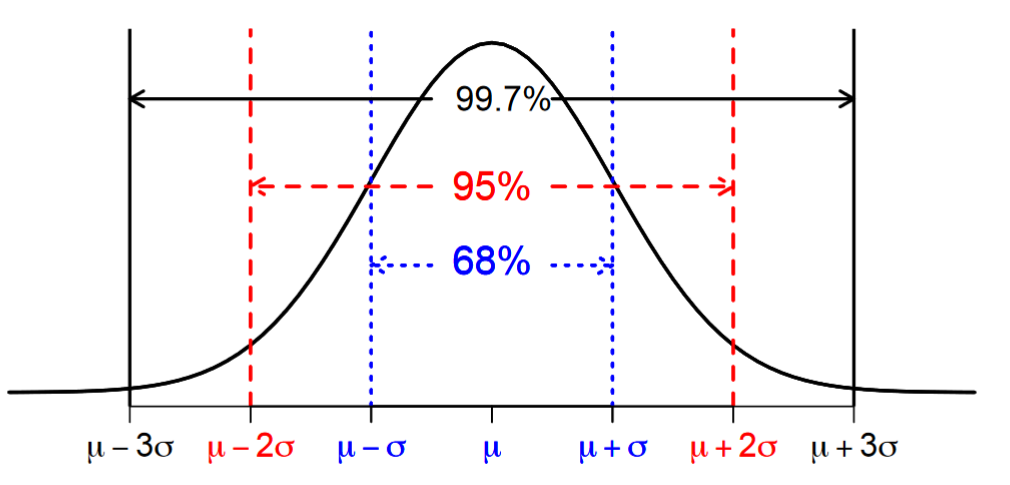
\includegraphics[width = 8cm]{Ch4NormalDist_StdDev}
\end{center}
\begin{equation*}
    \begin{aligned}
        \pm 1 \sigma :& P(\mu - \sigma < X < \mu + \sigma) = 0.6827 \\
        \pm 2 \sigma :& P(\mu - 2 \sigma < X < \mu + 2 \sigma) = 0.9545 \\
        \pm 3 \sigma :& P(\mu - 3 \sigma < X < \mu + 3 \sigma) = 0.9973 \\
    \end{aligned}
\end{equation*}

\subsubsection*{\textbf{Standard} Normal Distribution}
\begin{defn}
    \textbf{Standard normal random variable (Z)} \\
    A normal random variable with
    \begin{equation*}
        \begin{aligned}
            \mu  = 0 \quad \sigma ^2 = 1
        \end{aligned}
    \end{equation*}
    is called a standard normal random variable and is denoted as Z
\end{defn}

\begin{defn}
    \textbf{Cumulative Distribution Function (CDF) of a standard normal random variable}\footnote{Values are found in Appendix Table III} \\
    \begin{equation*}
        \begin{aligned}
            \Phi (z) = P(Z \leq z) = F(z)
        \end{aligned}
    \end{equation*}
\end{defn}

\subsubsection*{Standardizing}
Suppose $X$ is a normal random variable with mean $\mu$ and variance $\sigma^2$. \\
Then, 
\begin{equation*}
    \begin{aligned}
        P(X \leq x) &= P(\frac{X - \mu}{\sigma} \leq \frac{x - \mu}{\sigma}) \\
                &= P(Z \leq z)
    \end{aligned}
\end{equation*}
Where 
\begin{enumerate}
    \item $Z$ is a standard normal random value
    \item $z = \frac{x - \mu}{\sigma}$ is the z-value obtained by standardizing $X$.
    \item The probability is obtained by using Appendix Table III using $z = \frac{x - \mu}{\sigma}$
\end{enumerate}
\subsection*{Exponential Distribution (4.7-4.11)}


\end{document}